\documentclass[11pt]{article}
\usepackage{tikz}
\usepackage{amssymb}
\usepackage{geometry}
\geometry{letterpaper, landscape, margin=0.4in}
\usetikzlibrary{positioning, calc}

\begin{document}

\begin{center}
{\Huge \textbf{THE VAULTS BELOW}}\\[0.3em]
{\Large Level 2 --- Hekatos \& Illaktamus | 25 Keyed Areas}
\end{center}

\vspace{0.3em}

\begin{center}
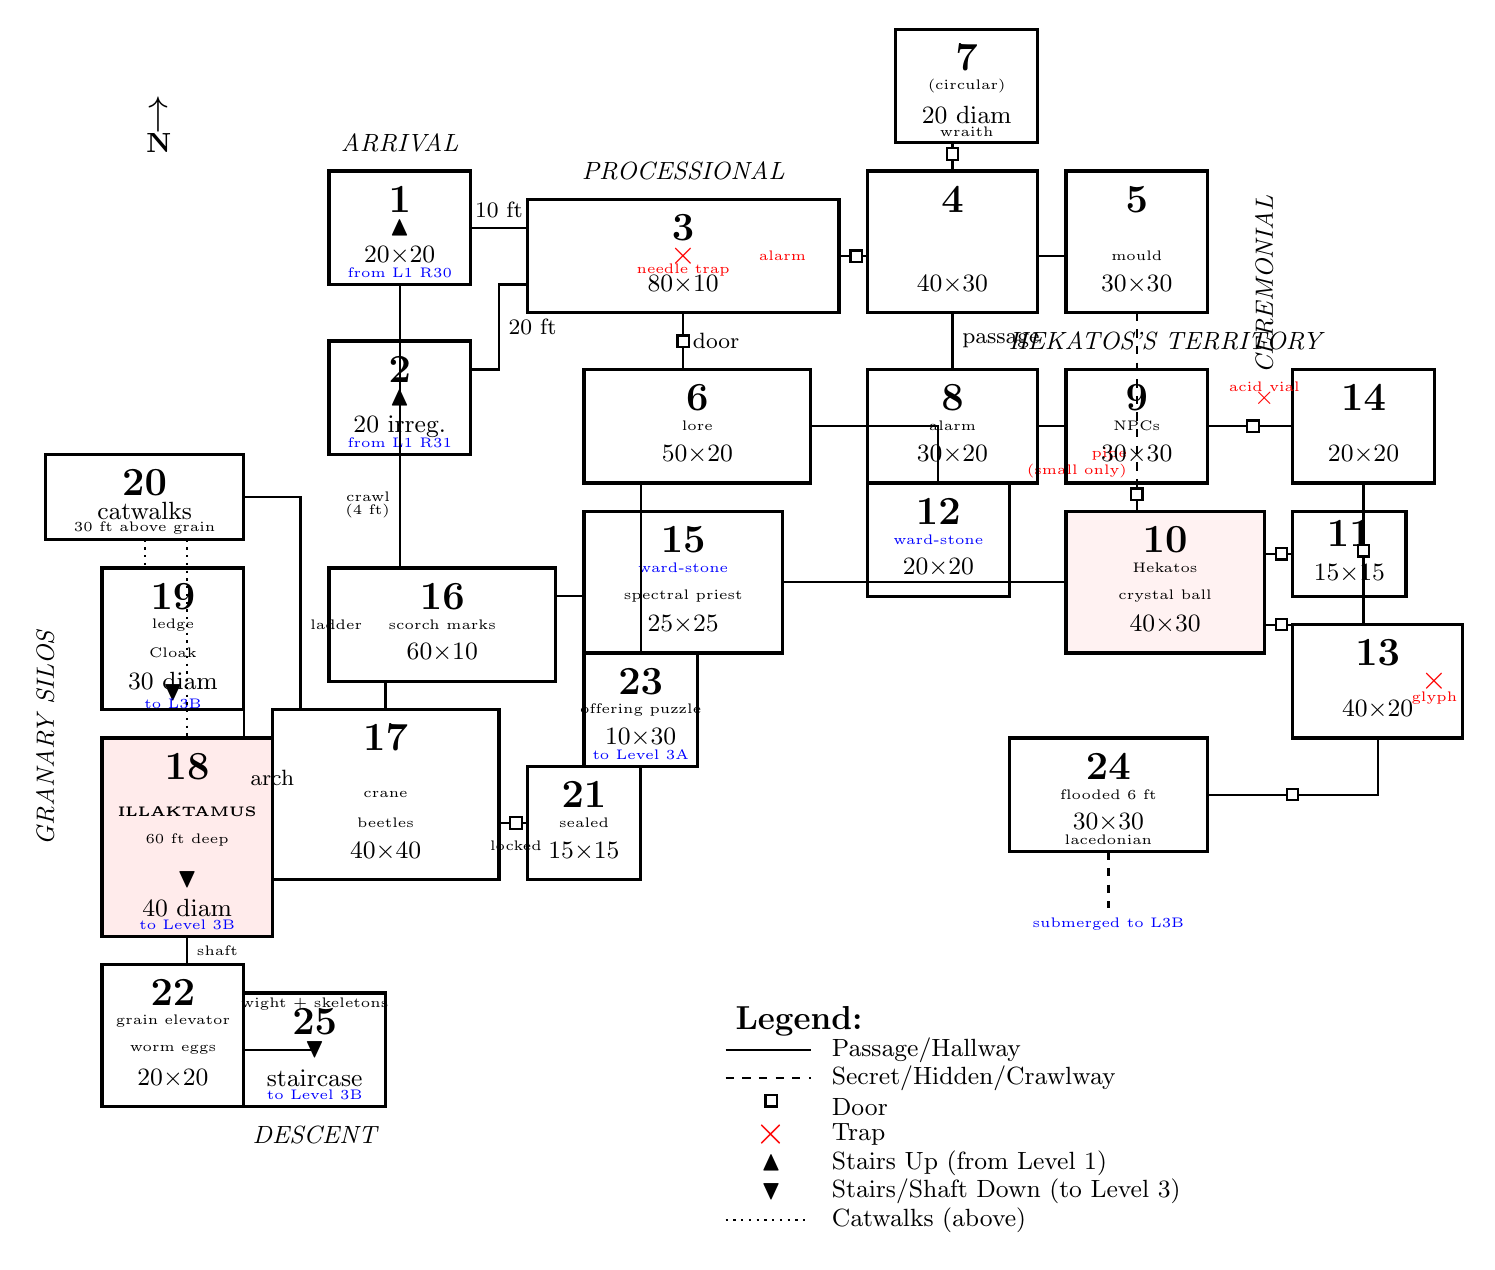
\begin{tikzpicture}[
    room/.style={draw, very thick, rectangle},
    connection/.style={draw, thick},
    door/.style={fill=white, draw=black, thick},
    secret/.style={dashed, thick},
    trap/.style={red},
    scale=0.72
]

% ============================================================
% NORTH ARROW
% ============================================================
\node at (-3,14) {\Large $\uparrow$};
\node at (-3,13.5) {\textbf{N}};

% ============================================================
% ARRIVAL & PROCESSIONAL (Rooms 1-3)
% ============================================================

% Room 1: Stair Landing (20x20)
\draw[very thick] (0,11) rectangle (2.5,13);
\node at (1.25,12.5) {\Large \textbf{1}};
\node[font=\small] at (1.25,11.5) {20$\times$20};
\node at (1.25,12) {$\blacktriangle$};
\node[font=\tiny,blue] at (1.25,11.2) {from L1 R30};

% Room 2: Collapsed Shaft (irregular 20 across)
\draw[very thick] (0,8) rectangle (2.5,10);
\node at (1.25,9.5) {\Large \textbf{2}};
\node[font=\small] at (1.25,8.5) {20 irreg.};
\node at (1.25,9) {$\blacktriangle$};
\node[font=\tiny,blue] at (1.25,8.2) {from L1 R31};

% Room 3: Processional Corridor (80x10)
\draw[very thick] (3.5,10.5) rectangle (9,12.5);
\node at (6.25,12) {\Large \textbf{3}};
\node[font=\small] at (6.25,11) {80$\times$10};

% Connection 1->3 (east)
\draw[thick] (2.5,12) -- (3.5,12);
\node[above,font=\footnotesize] at (3,12) {10 ft};

% Connection 2->3 (east)
\draw[thick] (2.5,9.5) -- (3,9.5) -- (3,11) -- (3.5,11);
\node[right,font=\footnotesize] at (3,10.25) {20 ft};

% Trap on Room 3 midpoint
\node[red] at (6.25,11.5) {\large $\times$};
\node[font=\tiny,red] at (6.25,11.25) {needle trap};

% Alarm ward near east end
\node[font=\tiny,red] at (8,11.5) {alarm};

% Connection 3->6 (south, midpoint door)
\draw[thick] (6.25,10.5) -- (6.25,9.5);
\node[right,font=\footnotesize] at (6.25,10) {door};
\fill[white,draw=black,thick] (6.15,9.9) rectangle (6.35,10.1);

% Connection 2->16 (south crawlway)
\draw[thick,dashed] (1.25,8) -- (1.25,6.5);
\node[left,font=\tiny] at (1.25,7.25) {crawl};
\node[left,font=\tiny] at (1.25,7) {(4 ft)};

% ============================================================
% CEREMONIAL CHAMBERS (Rooms 4-7)
% ============================================================

% Room 4: Robing Hall (40x30)
\draw[very thick] (9.5,10.5) rectangle (12.5,13);
\node at (11,12.5) {\Large \textbf{4}};
\node[font=\small] at (11,11) {40$\times$30};

% Connection 3->4 (east)
\draw[thick] (9,11.5) -- (9.5,11.5);
\fill[white,draw=black,thick] (9.2,11.4) rectangle (9.4,11.6);

% Room 5: Purification Baths (30x30)
\draw[very thick] (13,10.5) rectangle (15.5,13);
\node at (14.25,12.5) {\Large \textbf{5}};
\node[font=\small] at (14.25,11) {30$\times$30};
\node[font=\tiny] at (14.25,11.5) {mould};

% Connection 4->5 (east)
\draw[thick] (12.5,11.5) -- (13,11.5);

% Room 6: Hall of Inscriptions (50x20)
\draw[very thick] (4.5,7.5) rectangle (8.5,9.5);
\node at (6.5,9) {\Large \textbf{6}};
\node[font=\small] at (6.5,8) {50$\times$20};
\node[font=\tiny] at (6.5,8.5) {lore};

% Room 7: Vigil Chamber (20 diam circular)
\draw[very thick] (10,13.5) rectangle (12.5,15.5);
\node at (11.25,15) {\Large \textbf{7}};
\node[font=\small] at (11.25,14) {20 diam};
\node[font=\tiny] at (11.25,14.5) {(circular)};
\node[font=\tiny] at (11.25,13.7) {wraith};

% Connection 4->7 (north)
\draw[thick] (11,13) -- (11,13.5);
\fill[white,draw=black,thick] (10.9,13.2) rectangle (11.1,13.4);

% Connection 4->8 (south)
\draw[thick] (11,10.5) -- (11,9.5);
\node[right,font=\footnotesize] at (11,10) {passage};

% Connection 5->24 (pipe, secret)
\draw[thick,dashed] (14.25,10.5) -- (14.25,5.5);
\node[left,font=\tiny,red] at (14.25,8) {pipe};
\node[left,font=\tiny,red] at (14.25,7.7) {(small only)};

% ============================================================
% HEKATOS'S TERRITORY (Rooms 8-15)
% ============================================================

% Room 8: Outer Ward (30x20)
\draw[very thick] (9.5,7.5) rectangle (12.5,9.5);
\node at (11,9) {\Large \textbf{8}};
\node[font=\small] at (11,8) {30$\times$20};
\node[font=\tiny] at (11,8.5) {alarm};

% Connection 6->12 (east)
\draw[thick] (8.5,8.5) -- (9.5,8.5);
\node[above,font=\footnotesize] at (9,8.5) {};

% Room 9: Disciple Quarters (30x30)
\draw[very thick] (13,7.5) rectangle (15.5,9.5);
\node at (14.25,9) {\Large \textbf{9}};
\node[font=\small] at (14.25,8) {30$\times$30};
\node[font=\tiny] at (14.25,8.5) {NPCs};

% Connection 8->9 (east)
\draw[thick] (12.5,8.5) -- (13,8.5);

% Room 10: Research Chamber (40x30) -- Hekatos
\draw[very thick, fill=red!5] (13,4.5) rectangle (16.5,7);
\node at (14.75,6.5) {\Large \textbf{10}};
\node[font=\small] at (14.75,5) {40$\times$30};
\node[font=\tiny] at (14.75,6) {Hekatos};
\node[font=\tiny] at (14.75,5.5) {crystal ball};

% Connection 9->10 (south)
\draw[thick] (14.25,7.5) -- (14.25,7);
\fill[white,draw=black,thick] (14.15,7.2) rectangle (14.35,7.4);

% Room 11: Private Study (15x15)
\draw[very thick] (17,5.5) rectangle (19,7);
\node at (18,6.6) {\Large \textbf{11}};
\node[font=\small] at (18,5.9) {15$\times$15};

% Connection 10->11 (east/north)
\draw[thick] (16.5,6.25) -- (17,6.25);
\fill[white,draw=black,thick] (16.7,6.15) rectangle (16.9,6.35);

% Room 12: Second Ward-Stone (20x20)
\draw[very thick] (9.5,5.5) rectangle (12,7.5);
\node at (10.75,7) {\Large \textbf{12}};
\node[font=\small] at (10.75,6) {20$\times$20};
\node[font=\tiny,blue] at (10.75,6.5) {ward-stone};

% Connection 8->12 (south)
\draw[thick] (10.75,7.5) -- (10.75,7.5);

% Connection 6->12 (east from Hall of Inscriptions)
\draw[thick] (8.5,8.5) -- (10.75,8.5) -- (10.75,7.5);

% Room 13: Archives (40x20)
\draw[very thick] (17,3) rectangle (20,5);
\node at (18.5,4.5) {\Large \textbf{13}};
\node[font=\small] at (18.5,3.5) {40$\times$20};
\node[red] at (19.5,4) {\large $\times$};
\node[font=\tiny,red] at (19.5,3.7) {glyph};

% Connection 10->13 (east)
\draw[thick] (16.5,5) -- (17,5) -- (17,5);
\fill[white,draw=black,thick] (16.7,4.9) rectangle (16.9,5.1);

% Room 14: Alchemical Workshop (20x20)
\draw[very thick] (17,7.5) rectangle (19.5,9.5);
\node at (18.25,9) {\Large \textbf{14}};
\node[font=\small] at (18.25,8) {20$\times$20};

% Connection 9->14 (south from Disciples)
\draw[thick] (15.5,8.5) -- (17,8.5);
\fill[white,draw=black,thick] (16.2,8.4) rectangle (16.4,8.6);
\node[red] at (16.5,9) {\small $\times$};
\node[font=\tiny,red] at (16.5,9.2) {acid vial};

% Connection 13->14 (north)
\draw[thick] (18.25,5) -- (18.25,7.5);
\fill[white,draw=black,thick] (18.15,6.2) rectangle (18.35,6.4);

% Room 15: Third Ward-Stone (25x25)
\draw[very thick] (4.5,4.5) rectangle (8,7);
\node at (6.25,6.5) {\Large \textbf{15}};
\node[font=\small] at (6.25,5) {25$\times$25};
\node[font=\tiny,blue] at (6.25,6) {ward-stone};
\node[font=\tiny] at (6.25,5.5) {spectral priest};

% Connection 10->15 (south from Research Chamber)
\draw[thick] (13,5.75) -- (8,5.75);

% Connection 12->8 shared wall (already connected via the passage)

% ============================================================
% GRANARY SILOS (Rooms 16-22)
% ============================================================

% Room 16: Silo Approach (60x10)
\draw[very thick] (0,4) rectangle (4,6);
\node at (2,5.5) {\Large \textbf{16}};
\node[font=\small] at (2,4.5) {60$\times$10};
\node[font=\tiny] at (2,5) {scorch marks};

% Connection 1->16 (south from Stair Landing)
\draw[thick] (1.25,11) -- (1.25,6);
\node[left,font=\footnotesize] at (1.25,8.5) {};

% Connection 15->16 (west)
\draw[thick] (4.5,5.5) -- (4,5.5);

% Room 17: Loading Hall (40x40)
\draw[very thick] (-1,0.5) rectangle (3,3.5);
\node at (1,3) {\Large \textbf{17}};
\node[font=\small] at (1,1) {40$\times$40};
\node[font=\tiny] at (1,2) {crane};
\node[font=\tiny] at (1,1.5) {beetles};

% Connection 16->17 (west/south)
\draw[thick] (1,4) -- (1,3.5);

% Room 18: Upper Silo West (40 diam) -- ILLAKTAMUS LAIR
\draw[very thick, fill=red!8] (-4,-0.5) rectangle (-1,3);
\node at (-2.5,2.5) {\Large \textbf{18}};
\node[font=\small] at (-2.5,0) {40 diam};
\node[font=\tiny] at (-2.5,1.7) {\textbf{ILLAKTAMUS}};
\node[font=\tiny] at (-2.5,1.2) {60 ft deep};
\node at (-2.5,0.5) {$\blacktriangledown$};
\node[font=\tiny,blue] at (-2.5,-0.3) {to Level 3B};

% Connection 17->18 (west arch)
\node[font=\footnotesize] at (-1,2.3) {arch};

% Room 19: Upper Silo East (30 diam)
\draw[very thick] (-4,3.5) rectangle (-1.5,6);
\node at (-2.75,5.5) {\Large \textbf{19}};
\node[font=\small] at (-2.75,4) {30 diam};
\node[font=\tiny] at (-2.75,5) {ledge};
\node[font=\tiny] at (-2.75,4.5) {Cloak};
\node at (-2.75,3.8) {$\blacktriangledown$};
\node[font=\tiny,blue] at (-2.75,3.6) {to L3B};

% Connection 17->19 (west arch)
\draw[thick] (-1,3) -- (-1.5,3) -- (-1.5,3.5);

% Room 20: Silo Catwalks (walkways)
\draw[very thick] (-5,6.5) rectangle (-1.5,8);
\node at (-3.25,7.5) {\Large \textbf{20}};
\node[font=\small] at (-3.25,7) {catwalks};
\node[font=\tiny] at (-3.25,6.7) {30 ft above grain};

% Connection 17->20 (ladder up)
\draw[thick] (-0.5,3.5) -- (-0.5,7.25) -- (-1.5,7.25);
\node[right,font=\tiny] at (-0.5,5) {ladder};

% Connection 20 over 18 and 19 (catwalks span both silos)
\draw[thick,dotted] (-3.25,6.5) -- (-3.25,6);
\draw[thick,dotted] (-2.5,6.5) -- (-2.5,3);

% Room 21: Grain-Master's Vault (15x15)
\draw[very thick] (3.5,0.5) rectangle (5.5,2.5);
\node at (4.5,2) {\Large \textbf{21}};
\node[font=\small] at (4.5,1) {15$\times$15};
\node[font=\tiny] at (4.5,1.5) {sealed};

% Connection 17->21 (south, locked iron door)
\draw[thick] (3,1.5) -- (3.5,1.5);
\fill[white,draw=black,thick] (3.2,1.4) rectangle (3.4,1.6);
\node[below,font=\tiny] at (3.3,1.35) {locked};

% Room 22: Silo Floor Access (20x20)
\draw[very thick] (-4,-3.5) rectangle (-1.5,-1);
\node at (-2.75,-1.5) {\Large \textbf{22}};
\node[font=\small] at (-2.75,-3) {20$\times$20};
\node[font=\tiny] at (-2.75,-2) {grain elevator};
\node[font=\tiny] at (-2.75,-2.5) {worm eggs};

% Connection 18->22 (down through silo)
\draw[thick] (-2.5,-0.5) -- (-2.5,-1);
\node[right,font=\tiny] at (-2.5,-0.75) {shaft};

% ============================================================
% CONNECTING PASSAGES (Rooms 23-25)
% ============================================================

% Room 23: Sealed Passage (10x30)
\draw[very thick] (4.5,2.5) rectangle (6.5,4.5);
\node at (5.5,4) {\Large \textbf{23}};
\node[font=\small] at (5.5,3) {10$\times$30};
\node[font=\tiny] at (5.5,3.5) {offering puzzle};

% Connection 6->23 (west from Hall of Inscriptions)
\draw[thick] (5.5,7.5) -- (5.5,4.5);
\node[left,font=\footnotesize] at (5.5,6) {};

% Sealed wall annotation
\node[font=\tiny,blue] at (5.5,2.7) {to Level 3A};

% Room 24: Flooded Cistern (30x30)
\draw[very thick] (12,1) rectangle (15.5,3);
\node at (13.75,2.5) {\Large \textbf{24}};
\node[font=\small] at (13.75,1.5) {30$\times$30};
\node[font=\tiny] at (13.75,2) {flooded 6 ft};
\node[font=\tiny] at (13.75,1.2) {lacedonian};

% Connection 13->24 (south from Archives)
\draw[thick] (18.5,3) -- (18.5,2) -- (15.5,2);
\fill[white,draw=black,thick] (16.9,1.9) rectangle (17.1,2.1);

% Submerged passage to L3B
\draw[thick,dashed] (13.75,1) -- (13.75,0);
\node[below,font=\tiny,blue] at (13.75,0) {submerged to L3B};

% Room 25: Bone Stair (10 wide, descends 40 ft)
\draw[very thick] (-1.5,-3.5) rectangle (1,-1.5);
\node at (-0.25,-2) {\Large \textbf{25}};
\node[font=\small] at (-0.25,-3) {staircase};
\node at (-0.25,-2.5) {$\blacktriangledown$};
\node[font=\tiny,blue] at (-0.25,-3.3) {to Level 3B};
\node[font=\tiny] at (-0.25,-1.7) {wight + skeletons};

% Connection 22->25 (south/east passage)
\draw[thick] (-1.5,-2.5) -- (-0.25,-2.5);

% ============================================================
% WING LABELS
% ============================================================
\node[font=\small\itshape] at (1.25,13.5) {ARRIVAL};
\node[font=\small\itshape] at (6.25,13) {PROCESSIONAL};
\node[font=\small\itshape, rotate=90] at (16.5,11) {CEREMONIAL};
\node[font=\small\itshape] at (14.75,10) {HEKATOS'S TERRITORY};
\node[font=\small\itshape, rotate=90] at (-5,3) {GRANARY SILOS};
\node[font=\small\itshape] at (-0.25,-4) {DESCENT};

% ============================================================
% LEGEND
% ============================================================
\node[anchor=west,font=\large] at (7,-2) {\textbf{Legend:}};

\draw[thick] (7,-2.5) -- (8.5,-2.5);
\node[anchor=west,font=\small] at (8.7,-2.5) {Passage/Hallway};

\draw[thick,dashed] (7,-3) -- (8.5,-3);
\node[anchor=west,font=\small] at (8.7,-3) {Secret/Hidden/Crawlway};

\fill[white,draw=black,thick] (7.7,-3.5) rectangle (7.9,-3.3);
\node[anchor=west,font=\small] at (8.7,-3.5) {Door};

\node[red] at (7.8,-4) {\Large $\times$};
\node[anchor=west,font=\small] at (8.7,-4) {Trap};

\node at (7.8,-4.5) {$\blacktriangle$};
\node[anchor=west,font=\small] at (8.7,-4.5) {Stairs Up (from Level 1)};

\node at (7.8,-5) {$\blacktriangledown$};
\node[anchor=west,font=\small] at (8.7,-5) {Stairs/Shaft Down (to Level 3)};

\draw[thick,dotted] (7,-5.5) -- (8.5,-5.5);
\node[anchor=west,font=\small] at (8.7,-5.5) {Catwalks (above)};

\end{tikzpicture}
\end{center}

\vspace{0.5em}

\section*{Room Key}
\begin{small}
\begin{tabular}{rl|rl|rl}
1 & Stair Landing (20$\times$20) & 10 & Research Chamber (40$\times$30) & 19 & Upper Silo East (30 diam) \\
2 & Collapsed Shaft (20 irreg.) & 11 & Private Study (15$\times$15) & 20 & Silo Catwalks (walkways) \\
3 & Processional Corridor (80$\times$10) & 12 & 2nd Ward-Stone (20$\times$20) & 21 & Grain-Master's Vault (15$\times$15) \\
4 & Robing Hall (40$\times$30) & 13 & Archives (40$\times$20) & 22 & Silo Floor Access (20$\times$20) \\
5 & Purification Baths (30$\times$30) & 14 & Alchemical Workshop (20$\times$20) & 23 & Sealed Passage $\rightarrow$ L3A \\
6 & Hall of Inscriptions (50$\times$20) & 15 & 3rd Ward-Stone (25$\times$25) & 24 & Flooded Cistern (30$\times$30) \\
7 & Vigil Chamber (20 circ.) & 16 & Silo Approach (60$\times$10) & 25 & Bone Stair $\rightarrow$ L3B \\
8 & Outer Ward (30$\times$20) & 17 & Loading Hall (40$\times$40) & & \\
9 & Disciple Quarters (30$\times$30) & 18 & Upper Silo West (40 diam) & & \\
\end{tabular}
\end{small}

\section*{Connections to Other Levels}
\begin{small}
\begin{itemize}
    \item \textbf{Room 1 (Stair Landing):} Stairs up to Level 1, Room 30 (Grand Staircase)
    \item \textbf{Room 2 (Collapsed Shaft):} Climbing shaft up to Level 1, Room 31 (Collapsed Passage)
    \item \textbf{Room 18/19 (Grain Silos):} Shafts descend 30 ft through grain to Level 3B caverns
    \item \textbf{Room 22/25 (Silo Floor / Bone Stair):} Stone passages descend to Level 3B
    \item \textbf{Room 23 (Sealed Passage):} Blocked route to Level 3A (offering puzzle bypasses wall)
    \item \textbf{Room 24 (Flooded Cistern):} Submerged tunnel to Level 3B (requires water breathing)
\end{itemize}
\end{small}

\end{document}
